\chapter{Les relations islamo-chrétiennes sous les Abbassides}

\section{Bibliographie}

\begin{itemize}
    \item 
CAHEN Claude,
Islam, des origines au début de l’Empire ottoman , Paris,
Hachette, coll. « Pluriel », 2011.
    \item 
HOURANI Albert,
Histoire des peuples arabes , Paris, Seuil, coll. « Points »,
1993.
    \item 
LEWIS Bernard,
Les Arabes dans l’histoire , Paris, Flammarion, « Champs »,
1993.
    \item 
RODINSON Maxime,
Les Arabes, Paris, PUF, coll. « Quadrige », 2002.
 
    \item \textbf{John Tolan}, spécialiste des \textit{Dhimmis} au Moyen-âge.
Par ce programme de recherche, a permis d'avancer sur le sujet.
\end{itemize}


\section{Les Empires musulmans : la umma éclatée}

\begin{figure}
    \centering
    \sidecaption{Florian Louis,
Atlas historique du
Moyen Orient , Paris, Autrement,
2020, p. 39.}
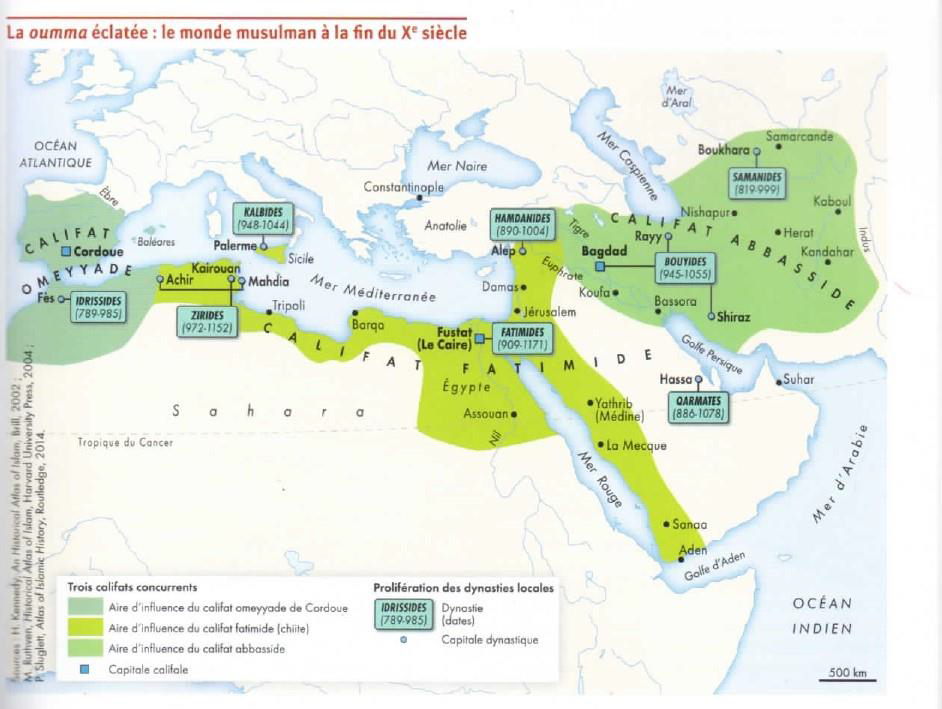
\includegraphics[width=0.8\textwidth]{HistoireIslamMediterranee/Images/SunnismeEclateX.png}
    \label{fig:my_label}
\end{figure}

\paragraph{Pourquoi un changement de régime} d'abord des raisons militaires avec des défaites (750)= face aux abbassides, mais aussi des mécontentements contre les Ommeyyades (les \textit{mawalis}, forte opposition). 

Diverses interprétations : 
\begin{itemize}
\item les orientalistes disent que c'est une opposition entre persans et arabes.
    \item Bernard Lewis : difficile d'accepter la position des orientalistes car ils projettent leurs visions nationalistes du XIXe.
    \item dimension religieuse. en particulier insiste Claude Cahin : plus du chisme religieux que Bernard Lewis. 
\end{itemize}

\begin{Synthesis}
Au dela des raisons militaires, il n'y a pas consensus sur les raisons, religieuses ou oppositions entre mawalis et arabes.
\end{Synthesis}

\paragraph{750 : début de l'empire abbasside} Transfert de la capitale à Bagdad. Ville carrefour commercial permettant de relier via l'intérieur des terres \Med à l'Inde : importance de la mésopotamie. \mn{repères chronologiques : 

Apogée de l’Empire abbasside sous le règne d’
Harun al Rachid (786
809)
 
Apogée de la puissance des Omeyyades en Espagne sous le règne du
calife Abd al Rahman III (912 961) => califat omeyyade en Espagne à
partir du Xe siècle
 
Création de la dynastie fatimide en Tunisie à partir de 910 puis
occupation de l’Egypte en 956 => califat fatimide}

\paragraph{Transformation des modes de succession} Mécontentement de la succession califaire qui serait dynastique : comment intégrer mawalis, esclaves ?...


\paragraph{Une organisation avec une bureaucratie reprise sur le monde perse} ministère, les \textit{diwans} : chancellerie. Des fonctionnaires pour faire tourner la bureaucratie. Des forces armées aussi organisées.  Comme tout empire, découpage de l'espace en province avec un gouverneur, l'\textit{émir}. Et pour la partie financière, l'\textit{amil}\sn{Les Abbassides reprennent les traditions administratives des sassanides. L’administration centrale est formée de bureaux ou offices (diwan) tenus par un corps de secrétaires (kuttab) : le bureau de l’impôt foncier (diwan al kharâdj), le bureau des domaines (diwan al diya), le bureau du Trésor (bayt al Mal), le bureau de la chancellerie (diwan al rasail), le bureau de l’armée (diwan al djaish). La poste (barid) a un rôle très important de communication et de renseignement. Les provinces sont dirigées par des gouverneurs (Khatib, puis émir et wali). Au début de l’Empire, leur gouvernement est souvent de courte durée car ils sont tentés de s’enrichir très vite et sont dénoncés par les hommes de la poste. Les finances des provinces sont confiées à un directeur des impôts (amil), la justice dépend du cadi. }. L'idée est toujours de favoriser le lien entre local et central. Le renseignement est aussi mis en place, pour anticiper les révoltes. 

\paragraph{Emergence de nouvelles classes sociales} mieux rémunérés. L'Empire est riche économiquement. Canne à sucre, blé, or, fer,... Grâce à ces ressources, va pouvoir se développer.

\paragraph{de grands travaux d'irrigation} en reprenant et développant les techniques d'irrigation grecques. 

\paragraph{Une imposition forte} le Kharadj, la capitation pour les non-musulmans. D'où la fonction d'\textit{Amil} avec ses représentants locaux.

\paragraph{le Qadi, fonction de jugement religieux} séparé de l'émir.



\paragraph{un siècle de rayonnement} sous le règne d'Harun al-Rachid (786-809). A sa mort, on voit déjà des signes de fragilisation avec guerre fratricide entre ses enfants. 


\paragraph{Après Harun, des princes autonomes}  830 : Sicile, leur permet de monter en Italie. 

\paragraph{Al Andalous} en 756, deuxième étape de la prise de l'Espagne (première installation en 710, les Omeyyades en Espagne). Pourquoi ce deuxième prise ? Les Omeyyades chassés de Damas vont s'installer en Espagne et chasser les berbères qui contrôlaient l'Espagne. Jusqu'en 1331. D'abord avec le titre d'Emir : il ne veut pas rompre l'\textit{umma}. Mais après le X, il prend le titre de \textit{calife d'Espagne}. 

\paragraph{Le califat Fatimide } Au meme moment, il y a eu une autre dynastie, en Tunisie en 910, d'origine Chiite, qui va se proclamer calife (qui donnera le califat fatimide). Pour des raisons religieuses et politiques (ils ne veulent pas être un pouvoir local), ils vont en Egypte (956) et fondent le califat fatimide.   Ils vont calquer leur organisation sur le califat abbasside (viennent de la péninsule arabique, chiite, descendants d'Ali et Fatima). Ils ne vont pas imposer leur doctrine aux musulmans egyptiens qui vont rester sunnites.  Une vraie question de la raison de cette non-imposition de la foi chiite.

\paragraph{Revenons à l'Espagne} une cour, avec des esclaves venant de la mer noire. Une armée composite, développement des villes, agriculture de subsistance (avec les berbères), administration calquée sur les abbassides. Cour de savants, musiciens. Jusqu'au X. Eclate en \textit{Taifas}, petites principautés et dynasties locales. 

\paragraph{Indépendance du Maroc par rapport à l'Espagne Omeyyade} Fès. Avec les Idrissides. 






%\includegraphics{}
% -------------------------------------------------------------------------------------------------
\section{Des relations islamo-chrétiennes de nature diversifiée}
% -------------------------------------------------------------------------------------------------

\paragraph{division religieuse} D'un côté il n'y a pas de pression pour se convertir mais la seule division qui va rester, et qui va être légalisé, c'est la distinction musulman / non-musulman. 


% -------------------------------------------------------------------------------------------------
\subsection{Au coeur de l'Empire des Abbassides}

\paragraph{un monde où l'islam est prépondérant} caravansérail, développement de l'arabe,... Le temps scandé par les 5 appels à la prière, ramadan, calendrier musulman.  \sn{A la différence de l'Empire Ottoman, qui est aussi scandé par les temps juifs et chrétiens}. D'un règne à un autre, d'une région à l'autre, il peut y avoir des changements.

\paragraph{Distinction des Dhimmis} reste le même. Le statut implique protection. Cela ne sera pas toujours le cas. 

\paragraph{Asymétrie} Remi Brague insiste sur la relation d'asymétrie.  Des différences religieuses, des différences d'habits,... Il ne faut pas trop idéaliser le statut de minorité en monde musulman : infériorité.
Pendant les fêtes religieuses chrétiennes et juives, il y a souvent des débordements. 
\begin{Ex}
Riche marchand chrétien. 
\end{Ex}

Mais à remettre dans un contexte où il y a aussi intolérance vis à vis des Chiites, riches marchants musulmans au sein du monde musulman,  Il ne faut pas idéaliser. Le Kharaj, impôt foncier, est plus élevé pour les non musulmans, les habits avec des couleurs différentes, des rites autorisés, interdiction d'avoir une maison plus élevée qu'un musulman, monter à cheval...

\paragraph{place des musulmans}
VIII : Moins de 10\% de musulmans, plutôt modeste. A la fin du X, la grande partie de l'empire est devenue musulmane : échapper au statut du dhimmi. Rigidification du statut inférieur. Il n'y pas de politique de conversion à l'Islam mais on ne peut revenir à sa religion d'origine.  

\paragraph{des quartiers par communauté} On soupçonne que cela commence aux époques des abbassides. Limite des échanges. Et du division du travail. Reste à creuser le développement économie et commercial de l'empire Abbasside. Des échanges jusqu'en Chine, Byzance, Scandinavie,...
Par rapport à ce qui dit Pirenne de la séparation de la méditerranée, ce n'est pas tout à fait juste. Les juifs comme intermédiaires.
Les banquiers sont essentiellement chrétiens et juifs (mais des musulmans banquiers existent).


\paragraph{Langue arabe} L'arabe, langue de l'administration, juridique, littérature... A coté des autres langues qu'on parle dans l'Empire abbasside. Arabisation via l'administration et en même temps, interaction qui existe entre les différents monothéismes. 

\paragraph{Révolte} entre arabes et coptes contre le gouverneur.  Où ? Caire ? 





% -------------------------------------------------------------------------------------------------
\section{En terre chrétienne conquise}
\begin{figure}
    \centering
    \sidecaption{Florian Louis,
Atlas historique du
Moyen Orient , Paris, Autrement,
2020, p. 38.}
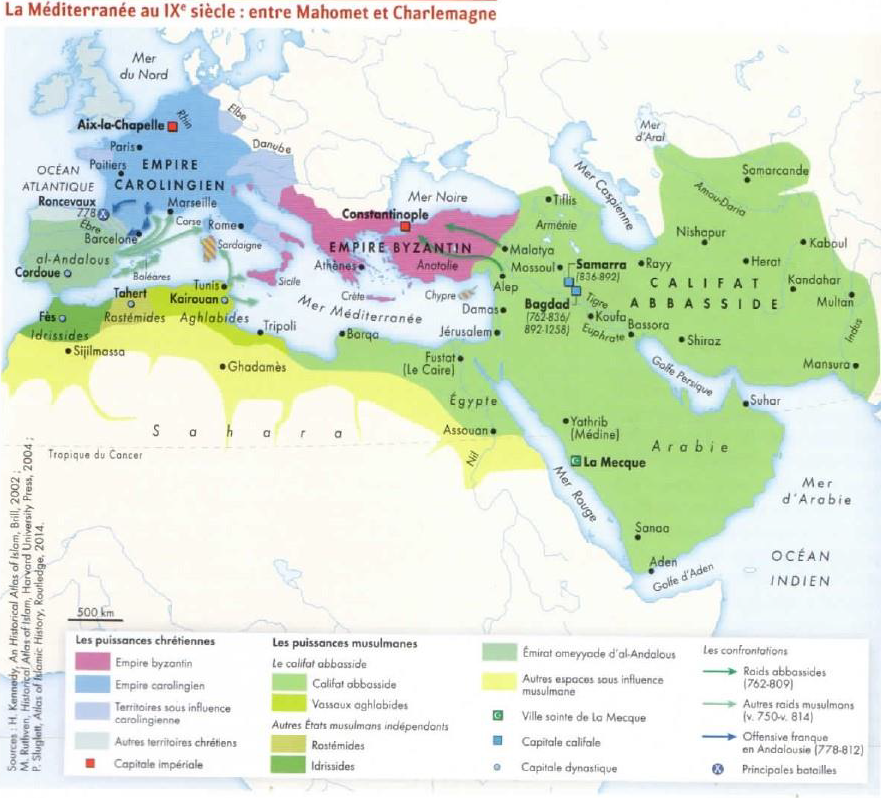
\includegraphics[width=0.8\textwidth]{HistoireIslamMediterranee/Images/MedIXe.png}
    \label{fig:my_label}
\end{figure}

 
\subsection{La Convivencia Espagnole}
\paragraph{la Convivencia} Espagnole. Mythe d'Al Andalus. Contrôle d'un pays essentiellement chrétien par des musulmans + berbere + esclave. Le statut de Dhimmi s'applique : 
\begin{itemize}
    \item pas de nouvelles eglises ni monastère
    \item pas de croix sur les Eglises, pas de cloche
    \item pas de procession
    \item pas de prière ostentatoire
    \item interdit vestimentaire, pas d'arme
\end{itemize}

John Tolan a montré que dans la pratique, quelques églises créées.

\paragraph{la cathédrale de Cordoue} partagée par les Chrétiens et les musulmans. l'Emir va acheter l'Eglise et va les autoriser à créer une nouvelle Eglise. 

\paragraph{fin X} majorité arabophone et musulmane. Raison : 
\begin{itemize}
    \item Attirance ? religieuse ? ou pas assez de prêtres ou Evèques ? face à ce vide, on se tournerait vers les musulmans
    \item échapper aux taxes
    \item statut privilégié. 
\end{itemize}


\paragraph{C'est trop pour le chrétien Alvaro ! Milieu du IXè}
\label{par:Alvaro}
\begin{quote}
    «
Beaucoup\sn{Cité par Bernard Lewis,
Les Arabes dans l’histoire , Paris, Flammarion, « Champs », 1993, p. 153.} de mes coreligionnaires lisent la poésie et les contes des Arabes ; ils
étudient les écrits des théologiens et des philosophes mahométans, non pour les
réfuter, mais pour apprendre comment s’exprimer eux mêmes en arabe avec une
correction et une élégance plus grandes. Où trouver aujourd’hui un laïc qui lise les
commentaires en latin sur les Saintes Ecritures ? Qui, parmi eux, étudie les Evangiles,
les Prophètes, les Apôtres ? Tous les jeunes chrétiens connus pour leurs talents ne
connaissent que la langue et la littérature des Arabes ; ils lisent et étudient avec zèle
les livres arabes, constituant à grands frais d’énormes bibliothèques et proclamant
partout, à qui veut les entendre, que cette littérature est digne d’admiration. Parmi des
milliers d’entre nous, à peine en trouve t on un qui sache écrire une lettre à un ami en
un latin passable, mais innombrables sont ceux qui peuvent s’exprimer en arabe et
composer de la poésie en cette langue, avec plus d’art que les Arabes eux mêmes. » 
\end{quote}

Pas le même statut entre Tolède, Seville et Cordoue, les autorités musulmanes entretiennent de bonnes relations vis à vis des autorités religieuses. Les Évêques sont validés par les Emirs. Que signifie la présence d'un Évêque à la cour ? 

\paragraph{la ville de Tolède} Arabisé mais restée chrétienne.  L'époque des Omeyyades et Taifas : ok convivencia mais après, ce n'est plus du tout le cas (Almoravides puis les Almohades, très rigoristes).

\paragraph{John Tolan : ne plus utiliser le terme de convivencia et aller au delà} Les Mozarabes, chrétiens arabisants. D'après les textes juridiques, charte urbaine (indiquant l'interdiction de fréquenter l'autre), cela veut dire que la pratique existe. L'image doit être nuancée. Modèle de cosmopolitisme / convivencia, est repris dans des unités politiques (dialogue Israel / Palestine, Chypre,...) : on va revenir sur cet âge d'or. 


\paragraph{vit on côte à côte} Il ne semble pas y avoir des quartiers spécifiques. Longue durée de la vie. Relation amicale avec quelqu'un d'une autre religion : dangereux pour les \textit{muftis} : interdiction des fêtes chrétiennes. Au même moment, le calife participe à une course équestre chrétienne. 
John Tolan : on ne fait pas appel à une nourrice juive ou chrétienne, on n'achète pas de la viande au boucher chrétien. Mariage mixte réglementé. On peut avoir des esclaves chrétiens.


\paragraph{Au quotidien vs texte législatif} Un \textit{Dhimmi} ne doit jamais avoir de pouvoir sur le musulman. Mais dans la pratique ? Attention, John Tolan travaille surtout sur la période post-abbasside. 

\paragraph{Tolède Chrétienne fin du XI} est aussi très tolérante. Accueille des musulmans pour les traductions.


\paragraph{Sicile Arabe} Une majorité reste chrétienne, jusqu'à la fin de la présence musulman. Certains \textit{dhimmis}, d'autres payent un \textit{tribu}. Pourquoi cette non conversion ? Le lien avec Bysance qui reste très fort ? Les architectes arabes vont beaucoup créer et resteront même quand la Sicile devient Normande : le géographe \textit{Idrissi}. Guillaume II, roi normand au XII (1166-1189), sait parler arabe. Il y a encore des documents et des monnaies en arabe sous le royaume normand.

\paragraph{histoire des langues} 


\begin{Synthesis}
    malgré les divisions, l'empire Abbasside est bien une économie-monde (au sens du Braudel) : ensemble cohérent unifié du point de vue économique. Circulent savoirs, techniques,...
    
\end{Synthesis}
